\documentclass[../main.tex]{subfiles}
%
\begin{document}
\chapter{Resultados}
A continuaci\'on relaciono los valores de los par\'ametros usados en todos los resultados siguientes:
\begin{table}[h]
	\centering
	\caption{Par\'ametros Hamiltonianos}
	\begin{tabular}{@{}l|l|l|l|l@{}}
		\toprule
		\textbf{Cavidad}              & \textbf{\begin{tabular}[c]{@{}l@{}}Punto \\ cu\'antico\end{tabular}} & \textbf{\begin{tabular}[c]{@{}l@{}}Bombeo \\ coherente\end{tabular}} & \textbf{\begin{tabular}[c]{@{}l@{}}Interacci\'on\\ electr\'on-fon\'on\end{tabular}} & \textbf{\begin{tabular}[c]{@{}l@{}}Campo\\ magn\'etico\end{tabular}} \\ \midrule
		$\omega_c = 1.00 \text{ meV}$ & $\delta_0 = 40.0 \text{ $\mu$eV}$                                    & $\Omega_1 = 82.0 \text{ $\mu$eV}$                                    & $g_{bb} = 20.0 \text{ $\mu$eV}$                                                     & $g_{hx} = -0.35$                                                     \\
		& $\delta_b = 18.0 \text{ $\mu$eV}$                                    & $\Omega_2 = 0.00 \text{ $\mu$eV}$                                    & $g_{bd} = g_{bb}$                                                                   & $g_{hz} = -2.20$                                                     \\
		& $\delta_d = 5.00 \text{ $\mu$eV}$                                    &                                                                      &                                                                                     & $g_{ex} = -0.65$                                                     \\
		&                                                                      &                                                                      &                                                                                     & $g_{ez} = -0.80$                                                     \\
		&                                                                      &                                                                      &                                                                                     & $\alpha = 20.0 \text{ $\mu$eV/T$^2$}$                                \\
		&                                                                      &                                                                      &                                                                                     & $\mu_B = 57.9 \text{ $\mu$eV/T}$                                     \\ \bottomrule
	\end{tabular}
\end{table}

\begin{table}[h]
	\centering
	\caption{Par\'ametros disipativos}
	\label{tab:my-table}
	\begin{tabular}{@{}l|l@{}}
		\toprule
		\textbf{Cavidad}                & \textbf{\begin{tabular}[c]{@{}l@{}}Punto \\ cu\'antico\end{tabular}} \\ \midrule
		$\kappa = 789 \text{ neV}$ & $\gamma_b = 18.7 \text{ neV}$                                     \\
		& $\gamma_d = 0.1 \gamma_b$                                            \\
		& $\gamma_\phi = 400 \text{ neV}$                                 \\ \bottomrule
	\end{tabular}
\end{table}

\section{Descomposici\'on espectral}

A continuaci\'on se muestra el espectro de energ\'ias del sistema cuando no hay campo magn\'etico ($B=0$), es decir, el sistema modelado por \cite{Vargas2022}. Se puede observar en la figura \ref{fig:energia-sin-campo-magnetico} que hay tres transiciones de estado permitidas y una prohibida a diferentes desafinamientos ($\Delta = \omega_b-\omega_L$) con $\omega_b$ siendo la energ\'ia de transici\'on del estado vac\'io ($\ket{v,0}$) al estado excit\'on brillante sim\'etrico ($\ket{X_{b+},0}$) y $\omega_L$ la energ\'ia del l\'aser. A continuaci\'on se muestran las transiciones permitidas con sus desafinamientos correspondientes y la transicion prohibida:
\begin{align}
	\bra{v,0}H\ket{X_{b+},2} &\neq 0 \quad \text{con} \quad \Delta \approx -2.001 \text{ meV},\\
	\bra{v,0}H\ket{X_{b-},2} &\neq 0 \quad \text{con} \quad \Delta \approx -1.981 \text{ meV},\\
	\bra{v,0}H\ket{X_{d+},2} &\neq 0 \quad \text{con} \quad \Delta \approx -1.957 \text{ meV},\\
	\bra{v,0}H\ket{X_{d-},2} &= 0 \quad \forall \;\; \Delta.
\end{align}

\begin{figure}[bh]
	\centering
	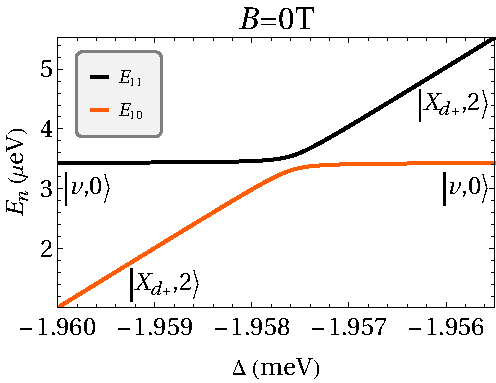
\includegraphics[width=.5\linewidth]{../res/E11E10_B0}
	\caption{Diagrama de energia del sistema cuando se gradua el laser de tal forma que al ir aumentando su frecuencia se encuentran transiciones entre estados cuya diferencia de variedades de excitacion es tres (gigante-Rabi), en este se muestran las tres permitidas y la prohibida. En la parte inferior se muestran los coeficientes de Hopfield del estado vacio con cada uno de los estados propios correspondientes.}
	\label{fig:E11E10_B0}
\end{figure}

Como se puede observar la interacci\'on es del orden de los $\mu$eV obteniendo que la intensidad de la interaccion es la diferencia entre las energias correspondientes. As\'i si se activa el campo magneticos vamos a ver en la figura \ref{fig:detuning-con-campo-magnetico} si el minimo (donde sucede la interaccion entre estados) sufre algun cambio.

\begin{figure}[bh]
	\centering
	\includegraphics[width=.9\linewidth]{../res/det_θ0}
	\caption{Desfinamiento $\Delta$ variando la magnitud del campo magnetico horizontal $\theta=0$ rad, para la gigante-Rabi de cada estado exciton, son cuatro posibles permitidos con diferencia tres entre sus variedades de excitacion, donde se observa que $\Delta$ depende del campo magnetico al cadradado, $\Delta \sim B^2$, con algunas transiciones involucran dependencia lineal del campo magnetico.}
	\label{fig:det_θ0}
\end{figure}

En la figura \ref{fig:detuning-con-campo-magnetico} se observa que el desafinamiento depende de la intensidad campo magnetico horizontal y es diferente para cada una de las transiciones permitidas, ademas, habilita la transicion prohibida anteriormente sin campo magnetico. A continuacion menciono la funcion numerica relacionado con el corrimiento del desafinamiento que me permite producir oscilaciones gigante Rabi con diferencia 3 en las variedades de excitacion:
\begin{align}
	\bra{v,0}H\ket{X_{b+},2} &\quad \text{con} \quad \textcolor{magenta}{\Delta \approx -2.001\text{ meV} - 0.025B - 0.02B^2},\\
	\bra{v,0}H\ket{X_{b-},2} &\quad \text{con} \quad \textcolor{blue}{\Delta \approx -1.981\text{ meV} - 0.01B - 0.02B^2},\\
	\bra{v,0}H\ket{X_{d+},2} &\quad \text{con} \quad \textcolor{darkgreen}{\Delta \approx -1.957\text{ meV} - 0.02B^2},\\
	\bra{v,0}H\ket{X_{d-},2} &\quad \text{con} \quad \textcolor{red}{\Delta \approx -1.954\text{ meV} + 0.018B - 0.02B^2}.
\end{align}


%
\end{document}